% ****** Start of file apssamp.tex ******
%
%   This file is part of the APS files in the REVTeX 4.2 distribution.
%   Version 4.2a of REVTeX, December 2014
%
%   Copyright (c) 2014 The American Physical Society.
%
%   See the REVTeX 4 README file for restrictions and more information.
%
% TeX'ing this file requires that you have AMS-LaTeX 2.0 installed
% as well as the rest of the prerequisites for REVTeX 4.2
%
% See the REVTeX 4 README file
% It also requires running BibTeX. The commands are as follows:
%
%  1)  latex apssamp.tex
%  2)  bibtex apssamp
%  3)  latex apssamp.tex
%  4)  latex apssamp.tex
%
\documentclass[%
% reprint,
%superscriptaddress,
%groupedaddress,
%unsortedaddress,
%runinaddress,
%frontmatterverbose, 
preprint,
%preprintnumbers,
%nofootinbib,
%nobibnotes,
%bibnotes,
 amsmath,amssymb,
 aps,
%pra,
%prb,
%rmp,
%prstab,
%prstper,
%floatfix,
]{revtex4-2}

\usepackage{graphicx}% Include figure files
\usepackage{dcolumn}% Align table columns on decimal point
\usepackage{bm}% bold math
%\usepackage{hyperref}% add hypertext capabilities
%\usepackage[mathlines]{lineno}% Enable numbering of text and display math
%\linenumbers\relax % Commence numbering lines

%\usepackage[showframe,%Uncomment any one of the following lines to test 
%%scale=0.7, marginratio={1:1, 2:3}, ignoreall,% default settings
%%text={7in,10in},centering,
%%margin=1.5in,
%%total={6.5in,8.75in}, top=1.2in, left=0.9in, includefoot,
%%height=10in,a5paper,hmargin={3cm,0.8in},
%]{geometry}
\usepackage{textgreek}
\usepackage{url}

\begin{document}

\preprint{}

\title{Potential involvement of the Frank-Starling mechanism in reduced stroke volume variability observed in a murine model of heart failure with reduced ejection fraction}% Force line breaks with \\
%\thanks{A footnote to the article title}%

\author{Gemma Fernández-Mendoza}
 \email{gemmag.fernandez@gmail.com}
\affiliation{%
 Departamento de Física, Escuela Superior de Física y Matemáticas, Instituto Politécnico Nacional, 07738 Ciudad de México, México
}%

\author{Hugo J. Alves-Figueiredo}
\email{dr.hugo_alves@tec.mx}
\affiliation{%
Cátedra de Cardiología y Medicina Vascular, School of Medicine and Health Sciences, Tecnologico de Monterrey, Monterrey, NL, Mexico
}%

\author{Gerardo García-Rivas}
\email{gdejesus@tec.mx}
\affiliation{%
The Institute for Obesity Research, Tecnologico de Monterrey, Monterrey, NL, Mexico.
}%

\author{Moisés Santillán}
 \homepage{http://moises-santillan.github.io}
 \email{msantillan@cinvestav.mx}
\affiliation{
 Centro de Investigación y de Estudios Avanzados, Unidad Monterrey, 66628 Apodaca NL, México
}%

\date{\today}% It is always \today, today,
             %  but any date may be explicitly specified

\begin{abstract}
Abnormal or reduced heart rate variability (HRV) is linked with conditions like chronic heart failure, diabetic neuropathy, and post-cardiac-transplant depression, among others. Such changes are associated with imbalances in the sympathetic and vagal nervous systems, which play a crucial role in regulating heart rate. However, other fundamental mechanisms that control the heart's contractile strength in vivo, including the Frank-Starling mechanism and the force-frequency relationship, have also been observed to change in patients with chronic heart failure. As a result, it is possible that other variables essential to heart function, such as stroke volume, may be impacted by these changes. To explore this possibility, we examined stroke volume variability (SVV) in a murine model of heart failure with reduced ejection fraction and found that SVV decreases in such condition. Our analysis of a simple cardiovascular system model suggests that the observed reduction in SVV may be due to changes in the Frank-Starling mechanism.
\end{abstract}

%\keywords{Suggested keywords}%Use showkeys class option if keyword
                              %display desired
\maketitle

%\tableofcontents

\section{\label{sec:intro}Introduction}

There is evidence that increased sympathetic nervous system activity is linked to increased cardiovascular morbidity and mortality \citep{Malpas_2010}. Concomitantly, the sympathetic and vagal nervous systems are key heart-rate regulators, and heart rate variability (HRV) analysis has been widely used as a noninvasive assessment tool for autonomic nervous system function \citep{Kiyono_2016}. Numerous results show that decreased and/or abnormal HRV is associated with conditions such as chronic heart failure, diabetic neuropathy, post-cardiac-transplant depression, fatigue severity in chronic fatigue syndrome, and susceptibility to sudden infant dead syndrome \citep{Kamen_1995, Rajendra_Acharya_2006, Zeki_Al_Hazzouri_2014, Escorihuela_2020}. 

Aside from the sympathetic and vagal nervous systems, the Frank-Starling mechanism and the force-frequency relationship are two basic mechanisms that regulate the heart's contractile strength in vivo \citep{Holubarsch_1996} , and changes in all of them have been reported in patients with chronic heart failure \citep{Mulieri_1992, Pieske_1992, Bristow_1982, Bristow_1989, Holubarsch_1996}. This raises the possibility that other variables, such as stroke volume, which are critical for heart function, may be altered in such pathology. This question is addressed in the present manuscript, using a murine model for heart failure with reduced ejection fraction.

\section{\label{sec:meth}Materials and Methods}

\subsection{Animal model of  Heart Failure with reduced ejection Fraction  (HFrEF)}

Mice with induced heart failure were used to study heart rate and stroke volume variability. C57BL/6 male mice weighing 20–30 g were randomly divided into two groups: a control group, and a heart-failure model group. During a week, the mice in the model group were given ad libitum access to drinking water supplemented with 1\% NaCl and 0.01\% of N-nitroL-arginine methyl ester (L-NAME). Following this, a micro-osmotic pump was surgically implanted into the subdermal dorsal area to release angiotensin II (ANGII) at a rate of 0.7 mg/kg/day, based on a prior report \citep{Ruiz_Esparza_2016}. On the other hand, the control group mice were provided plain water and underwent the same surgery but  did not have a pump implanted.

All animal experiments were reviewed and approved by the Institutional Animal Care and Use Committee of the Tecnológico de Monterrey in accordance with the NORMA Oficial Mexicana NOM-062-ZOO-1999. 

\subsection{Left-ventricle hemodynamics assessment}

At 28 days post-implantation of the pump, left-ventricle hemodynamics were evaluated in vivo using pressure-volume (PV) analysis with an open-heart configuration and the ADV500 PV measurement system (Transonic Scisense, NY, USA). A 1.2 Fr PV catheter was utilized for this purpose, following the methodology described in a prior publication \citep{Pacher_2008}.

\subsection{Fibrosis and cellular hypertrophy assessment}

After euthanizing the mice, their hearts were extracted and subjected to a semi-quantitative assessment of fibrosis and cellular hypertrophy, following \citet{Ruiz_Esparza_2016}. The samples were stained with Masson’s Trichrome or hemotosilin eosin and microphotographs were captured using an Imager Z.1 Zeiss microscope equipped with an AxioCam HRm camera. The microphotographs were processed using the AxioVision software. The PV records of mice with hearts that showed no signs of fibrosis and cellular hypertrophy indicative of heart failure were excluded from the study

\subsection{Variability analysis}

A variety of techniques have been used to measure variability. The vast majority of them are founded on the concept of signal stationarity. However, the heart's inherent non-stationary nature---which undergoes continuous physiological change to adapt to external stimuli---presents a significant challenge that could result in inaccurate results \citep{Marwan_2007}. Although several signal preprocessing methodologies have been proposed to address these issues, nonlinear analysis-based strategies are commonly employed and appear to produce reliable results. \citep{Marwan_2002, Aubert_2003, Marwan_2007, Giuliani_1998, 
Rajendra_Acharya_2006, Webber_1994, Henriques_2020}. One of them, used in different scientific domains is the Poincairé plot \citep{Hoshi_2016, Webber_1994, Voss_2008}. 

%The Poincaré plot is a graphical representation of a time series data that allows to visualize the dynamic patterns and the structure of variability in the system. It is named after the French mathematician Henri Poincaré, who first used it to study celestial mechanics.

The Poincaré plot is constructed by plotting the value of a given variable at time t+1 on the x-axis, against the value of the same variable at time t on the y-axis. Then, each point on the plot represents a pair of consecutive values of the variable, and the shape of the plot reflects the temporal dependencies and the non-linear dynamics of the system.

%In particular, the Poincaré plot can reveal information about the periodicity, the randomness, and the regularity of the data. For example, a circular shape of the plot indicates a periodic behavior, while a scattered or irregular shape suggests a more chaotic or random pattern. Additionally, the slope of the plot can indicate the rate of change or the directionality of the system.

In a Poincaré plot, there are two measures of the scatter of the data points (termed SD1 and SD2), which are used to quantify the dynamics of the system. SD1 is the standard deviation of the perpendicular distance of the data points to the line of identity (i.e., the line where the x and y values are equal, $y = -x$). SD1 is also known as the short-term variability, and it reflects the magnitude of the fluctuations of the system at a short time scale. In the particular case of heart-beat duration time-series, SD1 is related to the parasympathetic nervous system activity, which regulates the beat-to-beat changes in heart rate. SD2, on the other hand, is the standard deviation of the distances of the data points to the center of gravity of the plot, $y = x$. SD2 is also known as the long-term variability or the overall variability, and it reflects the magnitude of the fluctuations of the system at a longer time scale. In the case of heart rate variability, SD2 is related to the sympathetic nervous system activity \citep{Zimatore_2022}.

An algorithm was developed in \texttt{Python} to estimate the Poincaré-plot indices (SD1 and SD2) of heart-rate and stroke volume variability from time series data obtained experimentally. The algorithm has been made available for reference along with the experimentally recorded data at the following URL: \url{https://github.com/moises-santillan/HeartVariability}.

\subsection{Statistical analysis}

We conducted statistical analyses to detect significant differences between groups using Student's t-tests. To perform such analyses, we utilized the \texttt{ttest\_ind} function from the \texttt{scipy.stats} library in \texttt{Python}. Results with p-values less than 0.05 (type I error) were considered statistically significant.

\section{\label{sec:res}Results}

\subsection{\label{sec:conclu}Experimental results and heart variability analysis}

We conducted the experiments on the control and HFrEF groups according to the procedures outlined in Section Materials and Methods. From the recorded ventricle pressure and volume data we reconstructed for each experimental record the so-called P-V diagrams illustrated in Fig. \ref{fig:PVLoops}. Thereafter, we were able to extract time series of physiological interest from these diagrams, such as those of successive cardiac-cycle periods and stroke volumes.

\begin{figure}[h!]
    \begin{tabular}{cc}
        A & B \\
        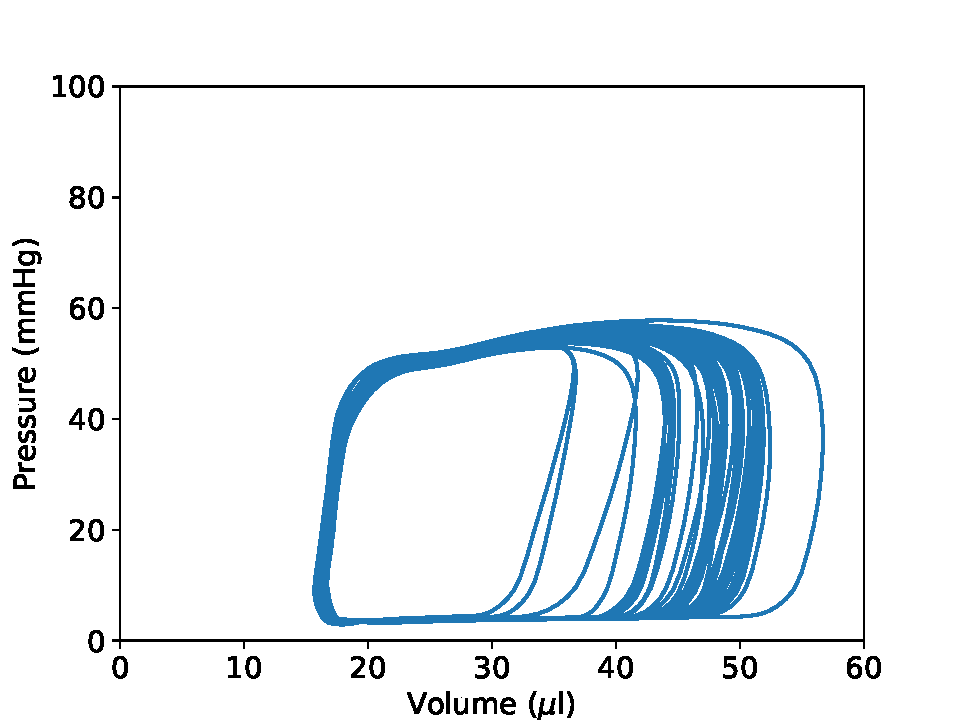
\includegraphics[width=3in]{PVLoops_A.pdf} &
        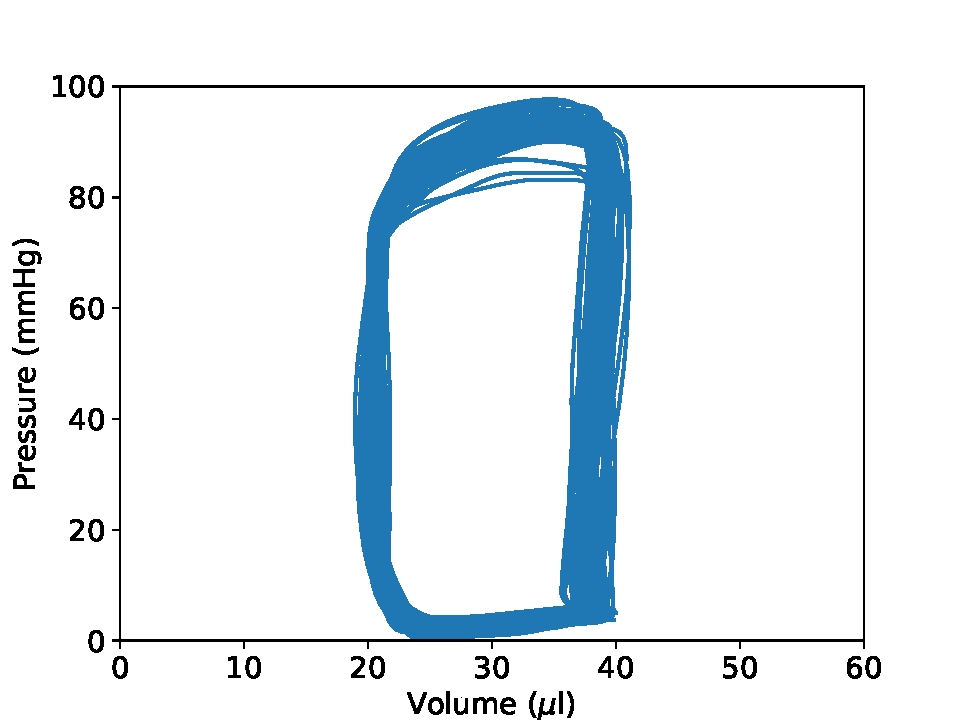
\includegraphics[width=3in]{PVLoops_B.pdf}
    \end{tabular}
    \caption{Sample PV loops recorded from a mouse in the control group (A) and a mouse in the HFrEF group (B).}
    \label{fig:PVLoops}
\end{figure}

The mean cycle duration was calculated for each experimental record by taking the time series of consecutive cardiac-cycle periods and averaging all of the values obtained in each group. Figure \ref{fig:fig01}A shows the results obtained. No significant difference was observed between the control group and the group of mice with induced cardiac failure, which contradicts the findings of \citet{Kamen_1995}, who found increased heart rates in patients with chronic heart failure. However, it is important to note that heart rate is controlled by the sympathetic and parasympathetic nervous systems. During the experiments, mice were anesthetized, which affects the autonomous nervous system. This may help explain the outcomes. Indeed, as noted by \citep{Nishiyama_2016, Kato_1992}, the employed anesthesia is known to affect heart rate.

\begin{figure}[h!]
    \begin{tabular}{cc}
        A & B \\
        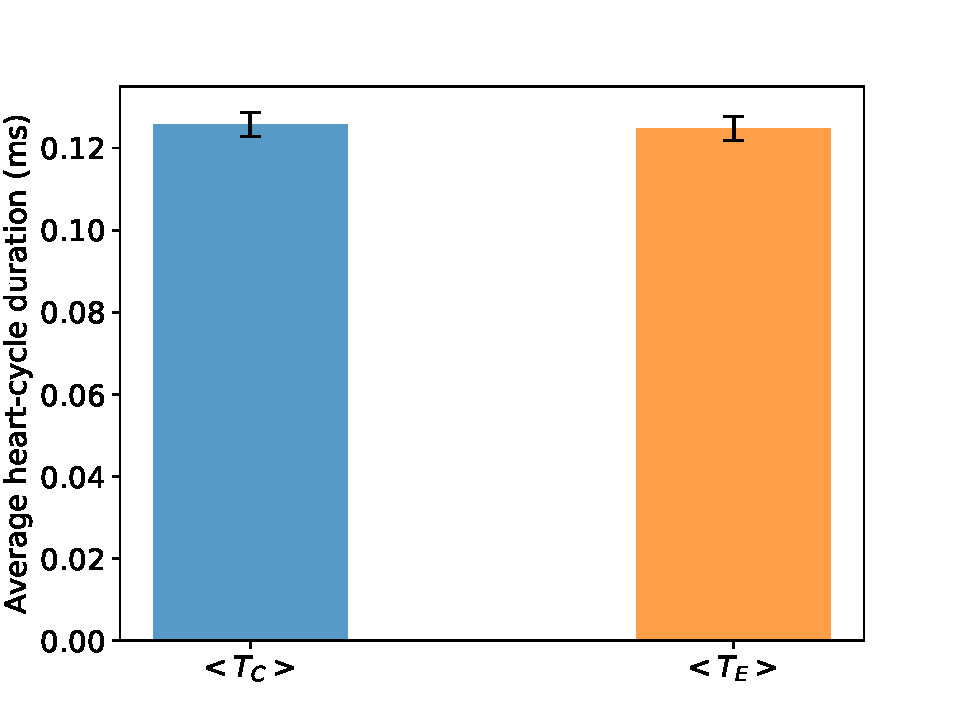
\includegraphics[width=3in]{Fig01_A.pdf} &
        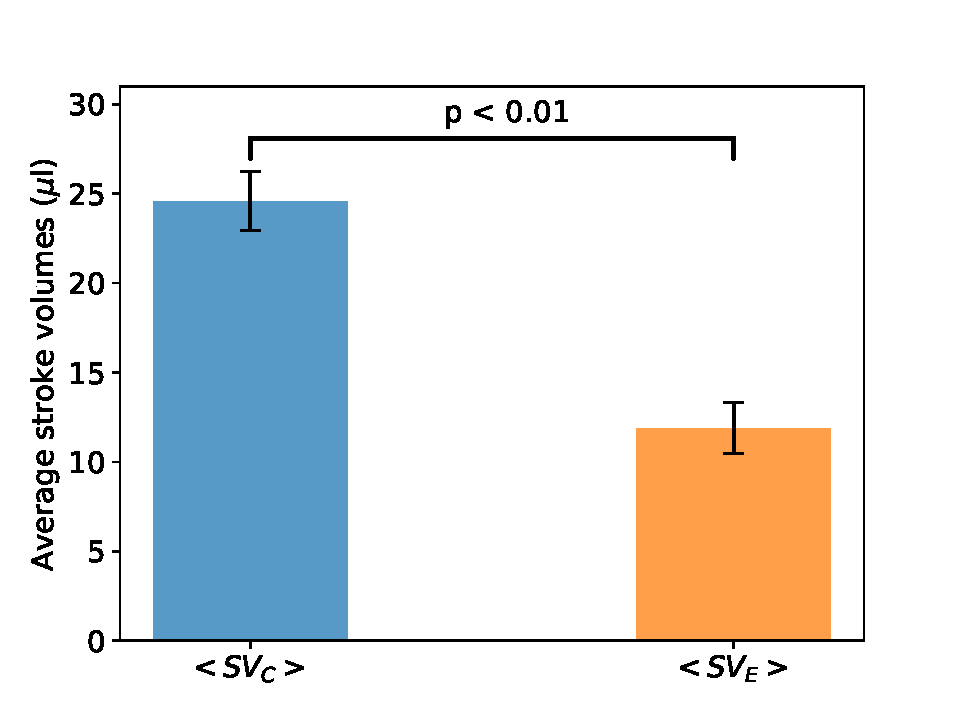
\includegraphics[width=3in]{Fig01_B.pdf}
    \end{tabular}
    \caption{A) Average cardiac-cycle periods for control (blue) and HFrEF (orange) groups. B) Average stroke volumes for control (blue) and HFrEF (orange) groups. Brackets indicates statistically significant difference.}
    \label{fig:fig01}
\end{figure}

We also calculated the mean values for the time series of consecutive stroke volumes for every experimental record. Then we averaged the results from each group and plotted the results in Fig. \ref{fig:fig01}B. As expected, there is a significant reduction in stroke volume in the group with induced heart failure when compared to the control group.

We were interested in studying the variability of heart-cycle periods and stroke volumes. Therefore, we measured the above described Poincaré-plot indices of heart-cycle period variability for every experimental record, and averaged the results corresponding to the control and HFrEF groups. The outcomes are plotted in Fig. \ref{fig:fig02}A. Observe that no statistically significant difference exists between the indices corresponding to the control and HFrEF groups. This suggests that, under our experimental conditions, heart failure does not affect heart rate variability (HRV). 

The same methodology was used to investigate the variability of stroke volumes. The results are shown in Fig. \ref{fig:fig02}B. The HFrEF group's SD1 and SD2 values are significantly lower than those of the control group. This, together with the absence of changes in HRV suggests that both types of variability are dissociated. Understanding why this happens is an intriguing question in itself. 

\begin{figure}[h!]
    \begin{tabular}{cc}
        A & B \\
        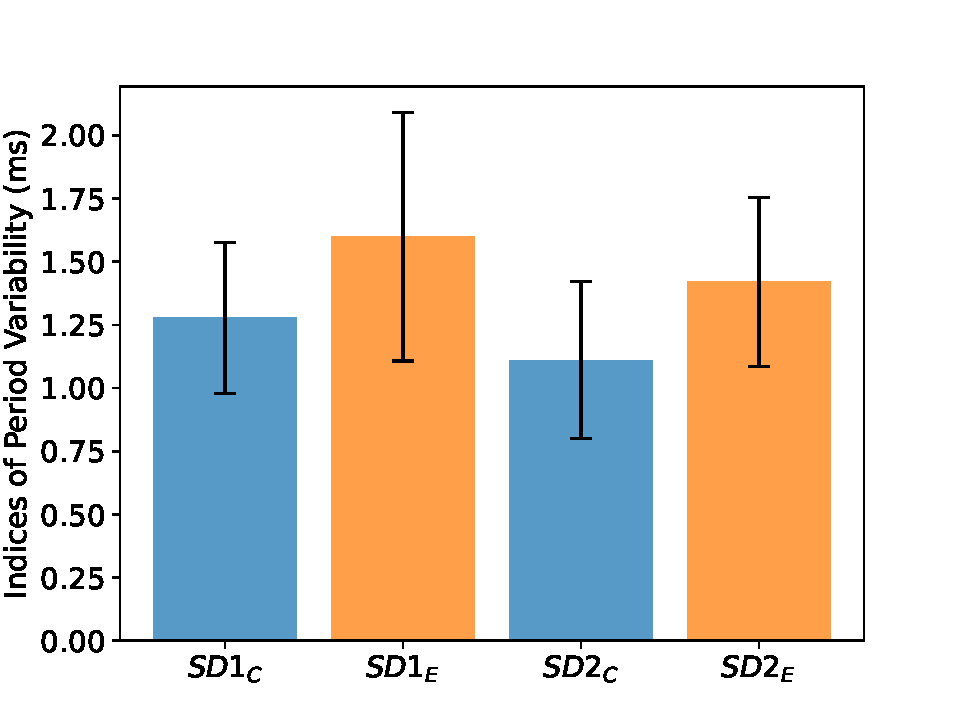
\includegraphics[width=3in]{Fig02_A.pdf} &
        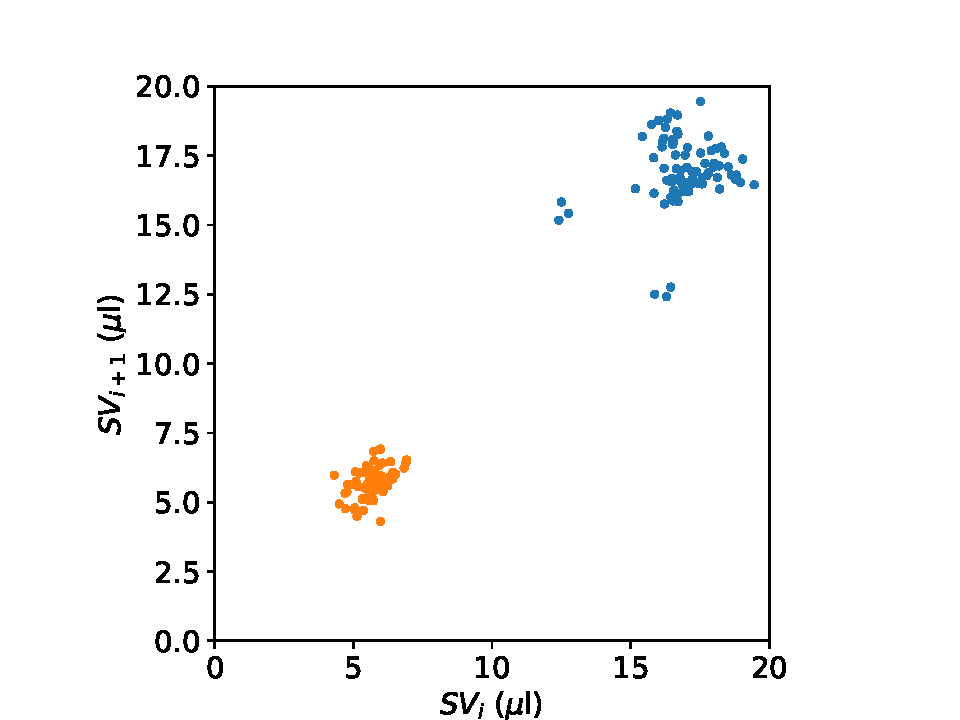
\includegraphics[width=3in]{Fig02_B.pdf}
    \end{tabular}
    \caption{A) Poincairé-plot indices of heart period variability for control (blue) and HFrEF (orange) groups. B) Poincairé-plot indices of stroke volume variability for control (blue) and HFrEF (orange) groups. Brackets indicates statistically significant difference.}
    \label{fig:fig02}
\end{figure}


We found that, in our experimental protocol, there is no difference in the heart rate of mice with induced heart failure compared to those in the control group. The same is true for heart rate variability (HRV). This last finding contradicts \citet{Kamen_1995} and other authors, who have reported that HRV decreases in patients with heart failure. We suggest that such discrepancy is related to the fact that mice are anesthetized in our experimental protocol. On the other hand, we found that, as expected, stroke volume decreases in mice with heart failure, as does stroke volume variability. 

As we mentioned before, HRV is a non-invasive tool that can provide valuable insights into the physiological state of an individual, including their stress levels, cardiovascular health, and risk of diseases such as diabetes and hypertension. Reduced HRV has been shown to be a strong predictor of cardiovascular events and mortality \citep{Zeki_Al_Hazzouri_2014}. We find it intriguing that the variability of stroke volume, which is also critical to heart function, is reduced in a pathology such as heart failure. What is more, our findings indicate that this decreased variability is caused by mechanisms other than those involved in HRV control. 

In order to gain some insight into this last question, we analyze in the following section a simple Frank-Starling model of the cardiovascular system that was previously introduced by \citet{Upton_2005}.

\subsection{Mathematical Model}

The model by \citeauthor{Upton_2005} is schematically represented in Fig. \ref{fig:model}. It separates the circulating blood into arterial and venous compartments. The pressure ($P_x$) and blood volume ($V_x$) in each compartment are related by the corresponding compliance ($C_x$):
\[
    P_x = V_x / C_x,
\] 
where subindex $x$ can have the values $A$ or $V$ to represent the arterial and venous compartments. The flow of blood from the arterial compartment to the venous compartment is assumed to be passive. Hence, the blood volume exchanged during period $\Delta t$ is:
\[
    V_R = \Delta t (P_A - P_V) / R,
\]
in which $R$ denotes the peripheral vascular resistance. Finally, to account for the Frank-Starling Law \citep{Jacob_1992}, the volume of blood transferred from the venous compartment to the arterial compartment by the heart pumping (stroke volume), is assumed to depend linearly on the venous pressure:
\[
    SV = \beta P_V.
\]
This is the model's most daring assumption, as it integrates the pulmonary circulation of blood and its passage through the heart auricles and ventricles in a single step.

\begin{figure}
\includegraphics[width=4in]{model.pdf}
\caption{Schematic representation of the Frank-Starling model of the cardiovascular system}
\label{fig:model}
\end{figure}

We now employ the \citeauthor{Upton_2005} model to investigate how the system's current state influences its evolution over successive cycles. To that end, we assume that the heart stroke occurs first, followed by passive diffusion of blood from the arterial compartment to the venous compartment. Let $V_{V,i}$ and $P_{V,i}$ denote the venous volume and pressure at the end of the $i$-th heart cycle. From this, the stroke volume in the next cycle is
\[
    SV_{i+1} = \beta P_{V,i}. 
\]
With this, the venous and arterial volumes after the heart stroke are:
\[
    V_{V, i+1/2} = V_{V, i} - SV_{i+1} \quad \text{and} \quad V_{A, i+1/2} = V_{A, i} + SV_{i+1}.
\]
After some algebra, these expressions can be rewritten as
\[
    V_{V, i+1/2} = V_{V,i} \left( 1 - \frac{\beta}{C_V} \right) \quad \text{and} \quad V_{A, i+1/2} = V_T - V_{V,i} \left( 1 - \frac{\beta}{C_V} \right),
\]
where $V_T$ is the total blood volume, which is assumed constant because the system is closed. After the heart stroke, a volume $V_{R, i+1}$ of blood passively diffuses back to the venous compartment. This volume is given by
\[
    V_{R, i+1} = \frac{1}{R}\left[ \frac{V_T}{C_A} - V_{V,i}\left(1-\frac{\beta}{C_V}\right)\left(\frac{1}{C_A} + \frac{1}{C_V}\right)\right].
\]
The venous and arterial volumes at the end of the $i+1$-th heart cycle can then be computed as:
\[
    V_{V, i+1} = V_{V,i} + V_{R, i+1} \quad \text{and} \quad V_{A, i+1} = V_{A,i} - V_{R, i+1}.
\] 
After performing the corresponding algebra, this last result leads to
\[
    V_{V, i+1} = V_{V,i} \left(1-\frac{\beta}{C_V}\right)\left[ 1 -\frac{1}{R}\left(\frac{1}{C_A} + \frac{1}{C_V}\right)\right] + \frac{V_T}{R C_A}.
\]
Finally, taking into account that $SV_{i+1} = \beta V_{V,i} / C_V$, it  follows that
\[
    SV_{i+1} = \mathcal{A} \, SV_{i}  + \mathcal{B},
\]
with
\begin{eqnarray*}
    \mathcal{A} & = & \left(1-\frac{\beta}{C_V}\right)\left[ 1 -\frac{1}{R}\left(\frac{1}{C_A} + \frac{1}{C_V}\right)\right], \\
    \mathcal{B} & = & \frac{V_T \beta}{R C_A C_V}.
\end{eqnarray*}
In other words, we derived a recursive expression for the stroke volume in consecutive heart cycles from the \citet{Upton_2005} model. It can be straightforwardly proved that such recursive equation converges to the stationary value
\[
    \overline{SV} = \frac{\mathcal{B}}{1 - \mathcal{A}},
\]
whenever $|\mathcal{A}| < 1$. Furthermore, the closer $\mathcal{A}$ is to 0, the faster the recursive equation converges to its stationary value.

The previous results imply that, when additive noise is included in the model, stroke volume variability is reduced for smaller $\mathcal{A}$ values. Take note, in particular, that $\mathcal{A}$ is a decreasing function of $\beta$. The decrease in short-term stroke volume variability observed in our experiments could then be explained by an increase in parameter $\beta$, which is related to the Frank-Starling mechanism. Interestingly, \citet{Holubarsch_1996} discovered, despite previous controversy, that the Frank-Starling mechanism is maintained in end-stage failing human hearts. They also found evidence that diastolic compliance was reduced in isolated preparations of failing human ventricles, indicating that higher end-diastolic stresses and pressures are required in failing hearts compared to normal hearts to achieve optimal contractile force. This might be translated into changes of parameter $\beta$ in our model and possibly explain the observed stroke volume variability.

\section{Concluding Remarks}

The available epidemiological and clinical data link increased sympathetic nervous system activity to increased cardiovascular morbidity and mortality, demonstrating that it has a strong predictive power for mortality and cardiovascular events \citep{Malpas_2010}. Heart rate variability (HRV) analysis has been widely used as a noninvasive assessment tool for autonomic nervous system function \citep{Kiyono_2016}, and results show that decreased and/or abnormal HRV is associated with conditions such as congestive heart failure, diabetic neuropathy, post-cardiac-transplant depression, fatigue severity in chronic fatigue syndrome, and susceptibility to sudden infant dead syndrome have been associated with modified (usually lower) heart rate variability \citep{Kamen_1995, Rajendra_Acharya_2006, Zeki_Al_Hazzouri_2014, Escorihuela_2020}. 

We found that stroke volume variability (SVV) decreases in a murine model for heart failure with reduced ejection fraction. Our results indicated that stroke volume variability is independent HRV, and the analysis of a simple model of the cardiovascular system suggests that the observed SVV reduction may be related to the Frank-Starling mechanism.

The Frank-Starling mechanism, along with the force-frequency relationship and the sympathetic and vagal nervous systems, is one of the basic mechanisms that regulate the contractile strength of the heart in vivo \citep{Holubarsch_1996}. Significant changes in the force-frequency relationship and the \textbeta-adrenoceptor system have been described in detail for failing human myocardium \citep{Mulieri_1992, Pieske_1992, Bristow_1982, Bristow_1989},  with the latter resulting in reduced HRV. However, this cannot explain SVV reduction in our experiments. Through a carefully planned set of experiments at the cell, organ, and organism levels, \citet{Holubarsch_1996} demonstrated that the Frank-Starling mechanism is well preserved in failing human myocardium. They also discovered significant changes in diastolic myocardial distensibility in patients with chronic heart failure. We speculate that these changes are at the root of the observed SVV reduction.

The findings presented in this paper should be approached with caution given the limitations of our methodology. While the absence of HRV in our experimental setup enabled us to establish that stroke volume variability is regulated by distinct mechanisms, it also restricts the generalizability of our results due to its departure from the typical physiological state. In addition, measurement introduces variability in our experimental setup, whether due to the movement/mechanical stability of a catheter placed in a beating heart or due to variability introduced by human error. To verify our findings, less intrusive methods of evaluating heart hemodynamics are necessary. The simplicity of our mathematical model is an additional constraint in our approach. However, creating and examining a more intricate model requires the estimation of model parameters from experimental data, some of which are not readily accessible in existing literature.

If further experimentation with appropriate setups validates our findings, it would give rise to several intriguing queries. For instance, what additional factors could potentially influence the reduction of variability in parameters such as SV? Would the variability of other parameters, such as injection fraction, also undergo changes? Could variability serve as an indicator of the severity of heart failure?

\begin{acknowledgments}
We wish to acknowledge Prof. Fernando Angulo-Brown for fruitful discussion and advice.
\end{acknowledgments}

\section*{Data availability statement}

The data that support the findings of this study are openly available at the following URL/DOI: \url{https://github.com/moises-santillan/HeartVariability}



\bibliography{manuscript}% Produces the bibliography via BibTeX.

\end{document}
%
% ****** End of file apssamp.tex ******
